\documentclass[fleqn, 12pt]{article}
\usepackage[0.7, swapVarGreek]{sigilz}
\usepackage{amssymb}
\usepackage{hyperref}
\usepackage{subdepth}

\setlength{\headheight}{15pt}
\pagestyle{fancy}
\lhead{Fei Yuan}
\chead{PHY905-004}
\rhead{Project}
\marginparsep=2cm

\begin{document}

\title{Project: parallel tensor contractions}
\date{2016-05-06}
\author{Fei Yuan}
\maketitle

\section{Background}

A \textit{tensor}, from a purely numerical perspective, is a multidimensional
array of numbers.  It is a generalization of matrices, which are
two-dimensional arrays.  Tensors arise naturally in quantum many-body
theories, including the in-medium similarity renormalization group (IM-SRG)
method -- one of the main methods that I develop as part of my research.

Many of the operations in IM-SRG involve computing summations of two tensors
over a subset of the indices, such as:
\begin{align}
  C_{i, j, k, l}
  &= \sum_{m = M_1}^{M_2} \sum_{n = N_1}^{N_2} A_{i, n, m, l} B_{m, j, k, n}
    \label{eq:a}
\end{align}
where $\bm A$, $\bm B$, and $\bm C$ are tensors and $M_1$, $M_2$, $N_1$, and
$N_2$ are some finite integers.  Summations of this form belong to a broad
family of operations called \textit{contractions}.

Similar to how tensors generalize matrices, contractions generalize matrix
multiplication.  For a binary contraction between two tensors $\bm A$ and
$\bm B$, we may partition the indices into three sets:
\begin{enumerate}
\item Free indices of $\bm A$ -- these appear on both sides of the equation and are not summed over.
\item Bound summation indices common to both $\bm A$ and $\bm B$.
\item Free indices of $\bm B$.
\end{enumerate}
If we label these sets of indices $I$, $J$, and $K$ respectively, we find a familiar equation:
\begin{align*}
  C_{I; K}
  &= \sum_J A_{I; J} B_{J; K}
\end{align*}
It is none other than matrix multiplication.  Mathematically, this appears to
be an elegant trick, but does it offer a practical advantage?

As it turns out, there is indeed an advantage in rewriting tensor contractions
in this form: matrix multiplication is a very well-studied problem, hence one
can save a great amount of development and computational time by taking
advantage of existing, highly-optimzied matrix libraries.

However, such an approach would require rewriting a tensor in a matrix form
specific to each type of contraction operation.  Computation-wise, this is
analogous to a \textit{transposition}, as it involves shuffling the tensor
elements around in memory.

This has both positive and negative consequences:
\begin{itemize}
\item Asymptotically, transpositions are generally cheaper than matrix
  multiplications, as the former only scales as the size of the tensor itself.
  Hence, one would expect its efficiency to be less crucial.
\item However, contractions tend to be quite cache-unfriendly due to their
  lack of temporal locality.  Even with blocking, which can be highly
  non-trivial for tensors with complicated symmetries, the best one can
  exploit is spatial locality.
\end{itemize}
This means in practice, the transposition portion can often be a significant
portion of the calculation time, even if its asymptotic scaling is better than
matrix multiplication.

The goal of this project is to develop an approach for performing the
transposition in a parallel and efficient manner.  The multiplication portion
is much simpler and well studied, hence it will not be the focus of this
project.

\section{Block-diagonal storage format}

Naive storage of the tensors that occur in many-body theory is generally
unfeasible as it would require terabytes of memory.  Fortunately, in most
problems there is some sort of conservation law (such as momentum
conservation) that manifests numerically as some additional, block-diagonal
structure in the matrix.

This generally means that a tensor contraction can be represented as the
multiplication of block-diagonal matrices, which trivially reduces to a
multiplication of each block separately, so in some sense it is analogous to a
vector of square matrices.

In a parallel system, a naive way to store these blocks would be to divide
them evenly between each node.  Unfortunately, the blocks generally occur in
wildly different sizes, hence some care is required in distributing these
blocks.

A simple algorithm for distributing objects of different sizes is the Longest
Processing Time (LPT) algorithm.  This algorithm makes a series of local
(greedy) decisions on which node gets to own which object, starting from the
largest object and ending at the smallest, taking care to always give the
object to the least occupied node.

The LPT algorithm works remarkably well in practice: distributing a set of
blocks of sizes $\{1^1, 2^2, \ldots, 100^2\}$ over 20 nodes yields a maximum
``imbalance'' of about $1\%$.  The imbalance $I$ is computed as:
\begin{align*}
  I = \frac{L_\text{max} - L_\text{min}}{L_\text{min}}
\end{align*}
where $L_\text{max}$ is the load of the most overloaded node and
$L_\text{min}$ is that of the least overloaded node.

\section{Transposing tensors in block-diagonal form}

In a typical many-body problem there would be many different kinds of tensor
contractions, some of which require incompatible block-diagonal structures.
The conversion between these structures constitutes the transposition part of
the tensor contraction algorithm, which involves performing a set of
complicated index computations.

From a high-level perspective, a transposition generally involves scattering
the elements of each block and reconstituting them into a completely different
blocks.  Without focusing on the details of specific physical problem, we can
simulate this movement as an essentially \emph{random} movement from one block
to another.

Concretely, suppose we have a list of $N$ blocks of different sizes that
represent a tensor $\bm C$.  Each block is labeled by an index $g$.  After
transposition, the tensor $\bm C$ is divided into $N'$ blocks of different
sizes, each labeled with $g'$.  Where a given element in the original tensor
goes is chosen from the uniform random distribution $g' \in [1, N']$.

In a sense, this can be thought of as the \emph{worst} case and least
cache-friendly scenario.  In a real problem, transposition is expected to
contain more structure than this, and therefore the results of this
measurement would be more of an empirical lower bound.

Similar to the initial distribution of the blocks, the blocks that appear
after the transposition also need to be distributed evenly across the nodes.
Here, however, it would be useful to reduce the amount of unnecessary movement
by attempting to allocate blocks on nodes that already contain a significant
fraction of the elements.

To accomodate this constraint, the LPT algorithm is modified so as to prefer
allocations that reduce unnecessary data movement by ``recycling'' from the
same node, without sacrificing the load balance.  This is accomplished by
allowing a nonzero \textit{tolerance} in the load of each node, so that if
some subset of nodes are within the tolerance of the least overloaded node,
then they are all eligible candidates for maximizing the number of elements
that are ``recycled''.  The parameter can be tuned manually and approximates
the allowable load imbalance.

Once computed by the root node, the distribution is then broadcast to all
other nodes so that the transposition may take place.  To avoid sending small
messages -- it would be quite costly to send each element as a single message
-- the elements are subdivided by their target block and packed using
MPI\textunderscore Pack.  Afterwards, each node performs an asynchonous send
and receive simultaneously with all other nodes and waits for completion.

\section{Results}

\begin{figure}
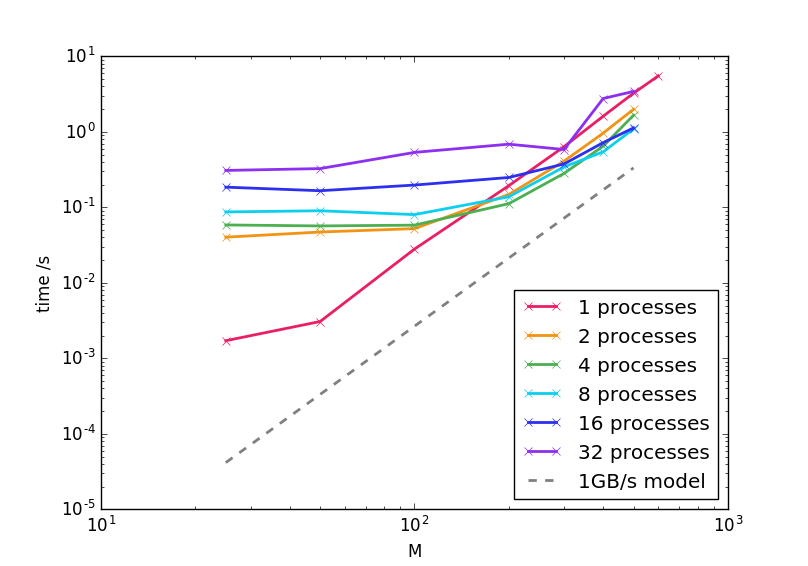
\includegraphics[width=\textwidth]{figure}
\caption{Time taken for the tensor transposition.}
\label{fig:1}
\end{figure}

For this project, we measure the time taken by the transposition for an
artificial tensor consisting of blocks of sizes $\{1^1, 2^2, \ldots, M^2\}$,
distributed over $N$ nodes.  The program was run on the MSU High Performance
Computing Center.

The results are plotted in Figure \ref{fig:1}.  A simple model is shown as
well for comparison, which is the amount of time it takes to transfer $M^3/3$
elements (the approximate sum of squares up to $M$) given a bandwidth of
$1\mathrm{GB/s}$.  The actual performance for the serial case is an order of
magnitude slower, indicating that the simple model was too optimistic.
Nonetheless, it predicts the overall trend of the serial case quite well.

The parallelized algorithms are noticeably slower for smaller quantities of
data (lower $M$), likely due to the communication and coordination overhead.
They do offer modest performance improvements for larger $M$, except for the
case with 32 processes which was almost entirely worse than serial.  It is
possible that with 32 processes some kind of serial bottleneck has been
reached, or that the quantity of data was still too small to make it
worthwhile.

\section{Conclusions}

In overall, the performance of the transposition was not stellar, but still
promising.  My original expectation was that it would perform worse, given the
additional overhead of passing messages around different nodes, the poor cache
locality in the transposition process, as well as the fact that the entire
transposition algorithm is communication bottlenecked.  Fortunately, it
appears that this is still worthwhile to do.

Moreover, even if the parallelized transposition is not particularly
beneficial by itself, it is still advantageous in some ways:
\begin{itemize}
\item Less memory on the nodes, allowing larger problems to be studied;
\item Parallelized matrix multiplication/tensor contraction.
\end{itemize}

I hope in the near future I can integrate this work into my production code
and further improve and analyze its performance.

The source code of the project can be found at: \url{https://github.com/xrf/phy905-proj}

\end{document}
